\documentclass[11pt,a4paper]{article}
\usepackage[margin=27mm]{geometry}
\usepackage{fontspec,booktabs,array,hyperref,graphicx}
\setmainfont{STIXGeneral}
\setlength{\parindent}{0pt}\setlength{\parskip}{5pt}
\begin{document}
\begin{center}{\Large Complete manuscript comparison}\\[3pt]
Overview v13: expanded projective and mixes topics\end{center}
The current comparison contains 19 topics and 46 recovered originals among 106 accessible originals; 60 remain pending and 55 earlier indexed originals remain archived. E now covers five originals, including L056 and L043, and Mixes covers F005 and L016. The other 17 topic records and 39 individual records retain their exact v12 boundaries, including the three symmetric listing corrections. Unified A and F007 are outside this edition.

The complete written factor is $\sum_i c(S_i)/(c(U)+\sum_i c(A_i))$ within each topic. Whole common theory and every complete local application are paid, without a cross-topic discount. Each row retains its adopted nonwhitespace-character coordinate. Expanded E uses raw-untrimmed NFC extraction, an explicit change from the earlier E coordinate; this primary was independently fixed and accepted. There is no pooled factor or inferred minimum proof complexity.
\begin{center}\small\begin{tabular}{lrrrrr}\toprule
Topic & Originals & Sources & Common & Applications & Factor\\\midrule
A & 7 & 213,803 & 49,059 & 87,019 & 1.571 \\
B & 5 & 124,906 & 44,905 & 69,265 & 1.094 \\
C & 5 & 118,433 & 30,437 & 61,248 & 1.292 \\
D & 3 & 47,894 & 15,632 & 29,855 & 1.053 \\
E & 5 & 140,286 & 57,473 & 32,337 & 1.562 \\
F & 2 & 69,825 & 15,876 & 27,398 & 1.614 \\
G & 2 & 73,199 & 30,928 & 85,207 & 0.630 \\
Affine & 1 & 32,767 & 19,070 & 22,638 & 0.786 \\
Representation & 1 & 25,348 & 11,288 & 13,688 & 1.015 \\
Chamber & 2 & 34,177 & 15,199 & 21,254 & 0.938 \\
Matching & 1 & 37,951 & 16,732 & 17,168 & 1.119 \\
ChiralEnumeration & 1 & 27,594 & 8,831 & 23,171 & 0.862 \\
Operations & 3 & 200,630 & 58,215 & 100,379 & 1.265 \\
Gluing & 1 & 27,081 & 28,416 & 11,565 & 0.677 \\
RankContraction & 1 & 15,530 & 6,937 & 10,555 & 0.888 \\
LocallyProjective & 2 & 26,490 & 25,498 & 11,966 & 0.707 \\
MathieuCensus & 1 & 13,736 & 5,516 & 35,862 & 0.332 \\
RankAugmentation & 1 & 33,604 & 13,904 & 14,096 & 1.200 \\
Mixes & 2 & 93,259 & 24,256 & 46,202 & 1.324 \\
\bottomrule\end{tabular}\end{center}
The exact \href{topics.csv}{19-topic CSV} and \href{applications.csv}{46-original CSV} preserve complete component costs, current fractions and historical observations. Factors below one remain visible. The accepted scientific source maps determine what each recovery covers; the numerical consolidation adds no separate proof or question credit.
\newpage
\section*{Individual comparisons: first 23 originals}
After acquiring the \emph{whole} common theory and all actual required mathematical, computational and data premises, the conditional factor is $c(S_i)/c(A_i)$. It charges the full local application or complete companion bundle. Optional validation is not silently made a theorem premise.
\begin{center}\small\begin{tabular}{llrrr}\toprule
Original & Topic & Source & Application & Factor\\\midrule
L032 & A & 16,558 & 8,212 & 2.016 \\
L034 & A & 21,433 & 5,784 & 3.706 \\
F016 & A & 43,983 & 15,419 & 2.853 \\
F013 & A & 25,562 & 6,224 & 4.107 \\
L035 & A & 51,019 & 14,498 & 3.519 \\
N009 & A & 36,824 & 28,114 & 1.310 \\
L128 & A & 18,424 & 8,768 & 2.101 \\
N001 & B & 14,519 & 7,371 & 1.970 \\
N003 & B & 17,780 & 9,155 & 1.942 \\
N008 & B & 18,009 & 11,132 & 1.618 \\
L030 & B & 22,704 & 12,286 & 1.848 \\
L040 & B & 51,894 & 29,321 & 1.770 \\
L088 & C & 13,166 & 11,311 & 1.164 \\
N013 & C & 27,361 & 15,815 & 1.730 \\
L108 & C & 12,849 & 10,075 & 1.275 \\
F014 & C & 20,577 & 6,962 & 2.956 \\
L068 & C & 44,480 & 17,085 & 2.603 \\
L066 & D & 20,916 & 10,989 & 1.903 \\
L074 & D & 20,661 & 13,367 & 1.546 \\
L104 & D & 6,317 & 5,499 & 1.149 \\
L079 & E & 21,212 & 1,858 & 11.417 \\
L083 & E & 20,904 & 2,922 & 7.154 \\
L021 & E & 29,594 & 14,452 & 2.048 \\\bottomrule\end{tabular}\end{center}
E pays its whole 20-page common paper, all five applications and all exact source qualifications. The five-source numerator uses 67 source pages. Application routes remain L083 to A1, L079 to A2, L021 to A3, L056 to A4 and L043 to A5. The broader quoted classifications and ancillary censuses remain retained where the source map says so; they are not newly claimed as regenerated results.

L043 names \emph{Magma} and the $L_2$-quotient algorithm. GAP and Python describe the replacement implementation. Its accepted corrections, L056's characteristic-two qualification, the L021 corrections, and the exclusion of L079's P$\Sigma$L$(2,25)$ clause remain explicit. E's 42 scoped Lean declarations are partial evidence, not full source formalization.
\newpage
\section*{Individual comparisons: remaining 23 originals}
\begin{center}\small\begin{tabular}{llrrr}\toprule
Original & Topic & Source & Application & Factor\\\midrule
L056 & E & 15,871 & 4,144 & 3.830 \\
L043 & E & 52,705 & 8,961 & 5.882 \\
L014 & F & 25,574 & 11,504 & 2.223 \\
L007 & F & 44,251 & 15,894 & 2.784 \\
L009 & G & 49,891 & 23,544 & 2.119 \\
L092 & G & 23,308 & 61,663 & 0.378 \\
L012 & Affine & 32,767 & 22,638 & 1.447 \\
F010 & Representation & 25,348 & 13,688 & 1.852 \\
L008 & Chamber & 20,159 & 7,571 & 2.663 \\
N016 & Chamber & 14,018 & 13,683 & 1.024 \\
F015 & Matching & 37,951 & 17,168 & 2.211 \\
L028 & ChiralEnumeration & 27,594 & 23,171 & 1.191 \\
N005 & Operations & 122,002 & 49,595 & 2.460 \\
N006 & Operations & 55,740 & 38,479 & 1.449 \\
N007 & Operations & 22,888 & 12,305 & 1.860 \\
L010 & Gluing & 27,081 & 11,565 & 2.342 \\
L037 & RankContraction & 15,530 & 10,555 & 1.471 \\
L084 & LocallyProjective & 2,071 & 4,857 & 0.426 \\
L095 & LocallyProjective & 24,419 & 7,109 & 3.435 \\
L073 & MathieuCensus & 13,736 & 35,862 & 0.383 \\
L020 & RankAugmentation & 33,604 & 14,096 & 2.384 \\
F005 & Mixes & 57,753 & 31,077 & 1.858 \\
L016 & Mixes & 35,506 & 15,125 & 2.348 \\\bottomrule\end{tabular}\end{center}
Mixes pays both complete common papers, with costs 12,615 and 11,641. F005's application pays both its main and exceptional papers (20,788 plus 10,289); L016's complete local paper costs 15,125. Both required finite certificates remain required, while four validation programs remain optional. Six scoped formal declarations do not formalize the full sources.

The three final F005 problems remain unanswered. L016's literal thin-cover Lemma 3.5 is corrected under faithfulness; Proposition 5.4 is stated without CIP. Ancillary smallest-example/Atlas census and further-cover questions remain outside the accepted principal recovery. A corrected source theorem is not assigned a new solved-question credit.

Executable listings are excluded symmetrically, while proof and mathematical algorithm prose remain. All required program/data and optional validation inventories are preserved separately. Historical software, external proofs, complete graphics and full formalization costs are unknown; software-inclusive and pooled factors remain null. Operations retains its separate text-only sensitivity. Prior overviews remain historical records.
\newpage
\section*{Whole topics}
Grey bars show the complete original manuscript text in each row's adopted coordinate. Replacement bars stack the entire common theory and every local application. The axis starts at zero; the tables contain ratios.
\begin{center}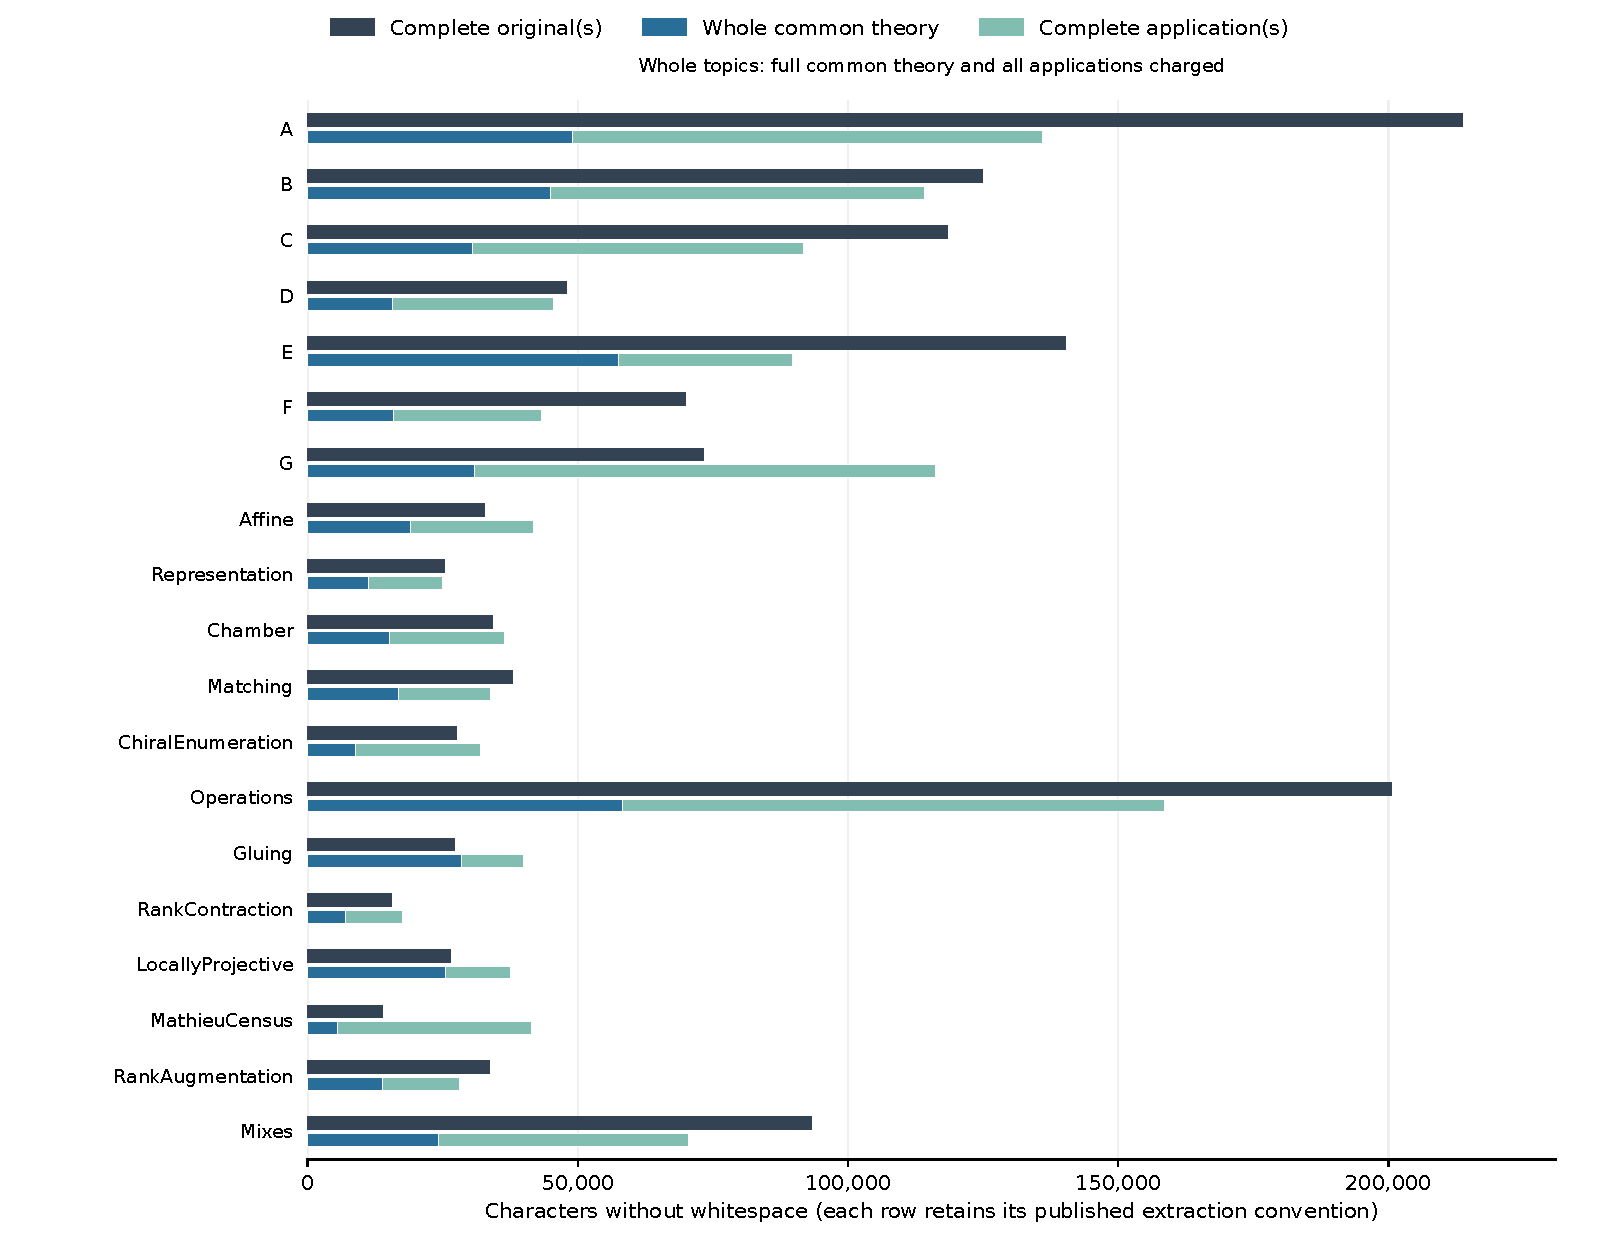
\includegraphics[width=\linewidth]{whole_topics.pdf}\end{center}
The 57 bars account for all 19 complete topics. Shared theory remains charged even when only some applications invoke a section. No required code or external premise is treated as mathematically unnecessary because its cost is outside the manuscript coordinate.
\newpage
\section*{Conditional lengths: first 23 originals}
Whole common theory and required premises are acquired in advance. Grey and teal bars compare complete source and local application text; these bars do not remove the prerequisite cost from the whole-topic table.
\begin{center}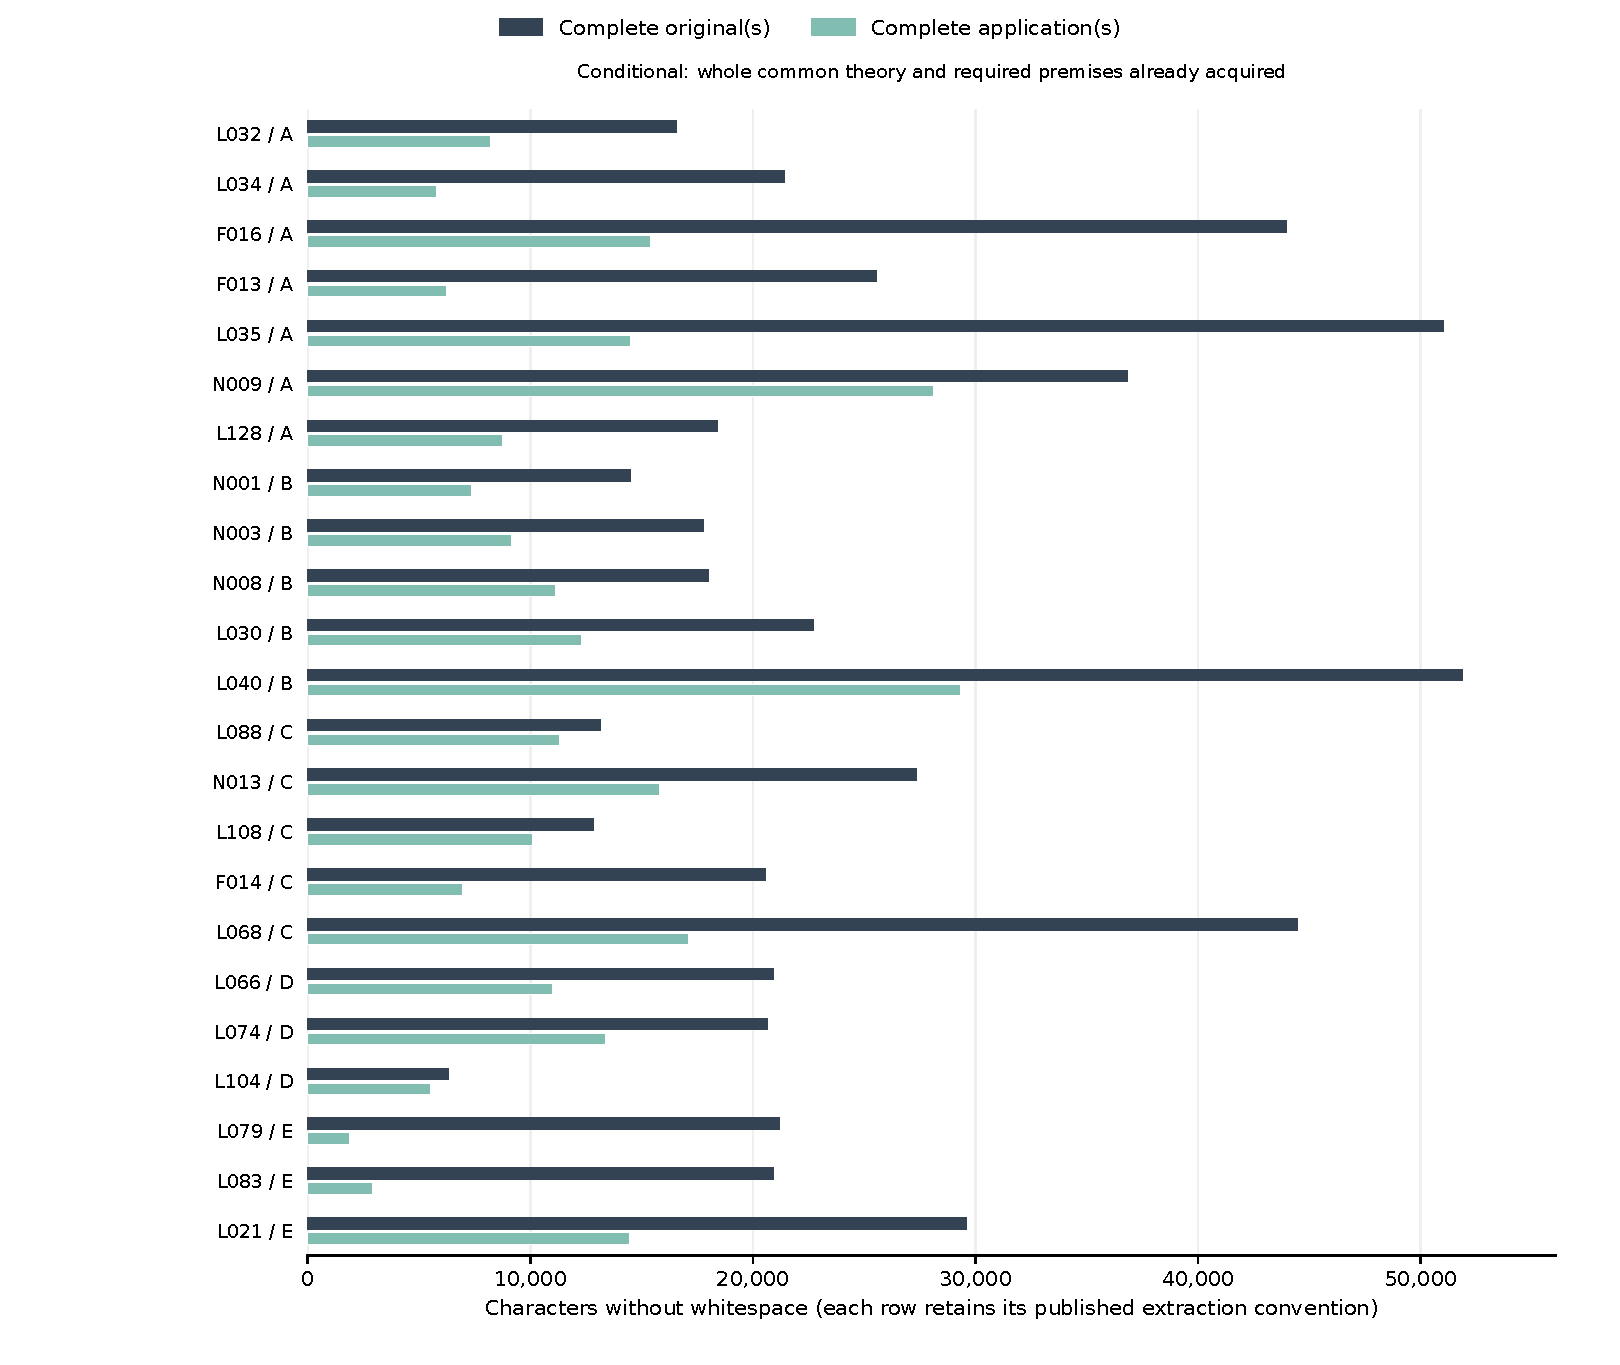
\includegraphics[width=\linewidth]{conditional_1.pdf}\end{center}
\newpage
\section*{Conditional lengths: remaining 23 originals}
All complete companion papers remain charged. The source sequence is documentary, with no optimized acquisition order, sawtooth or proof-node factor implied.
\begin{center}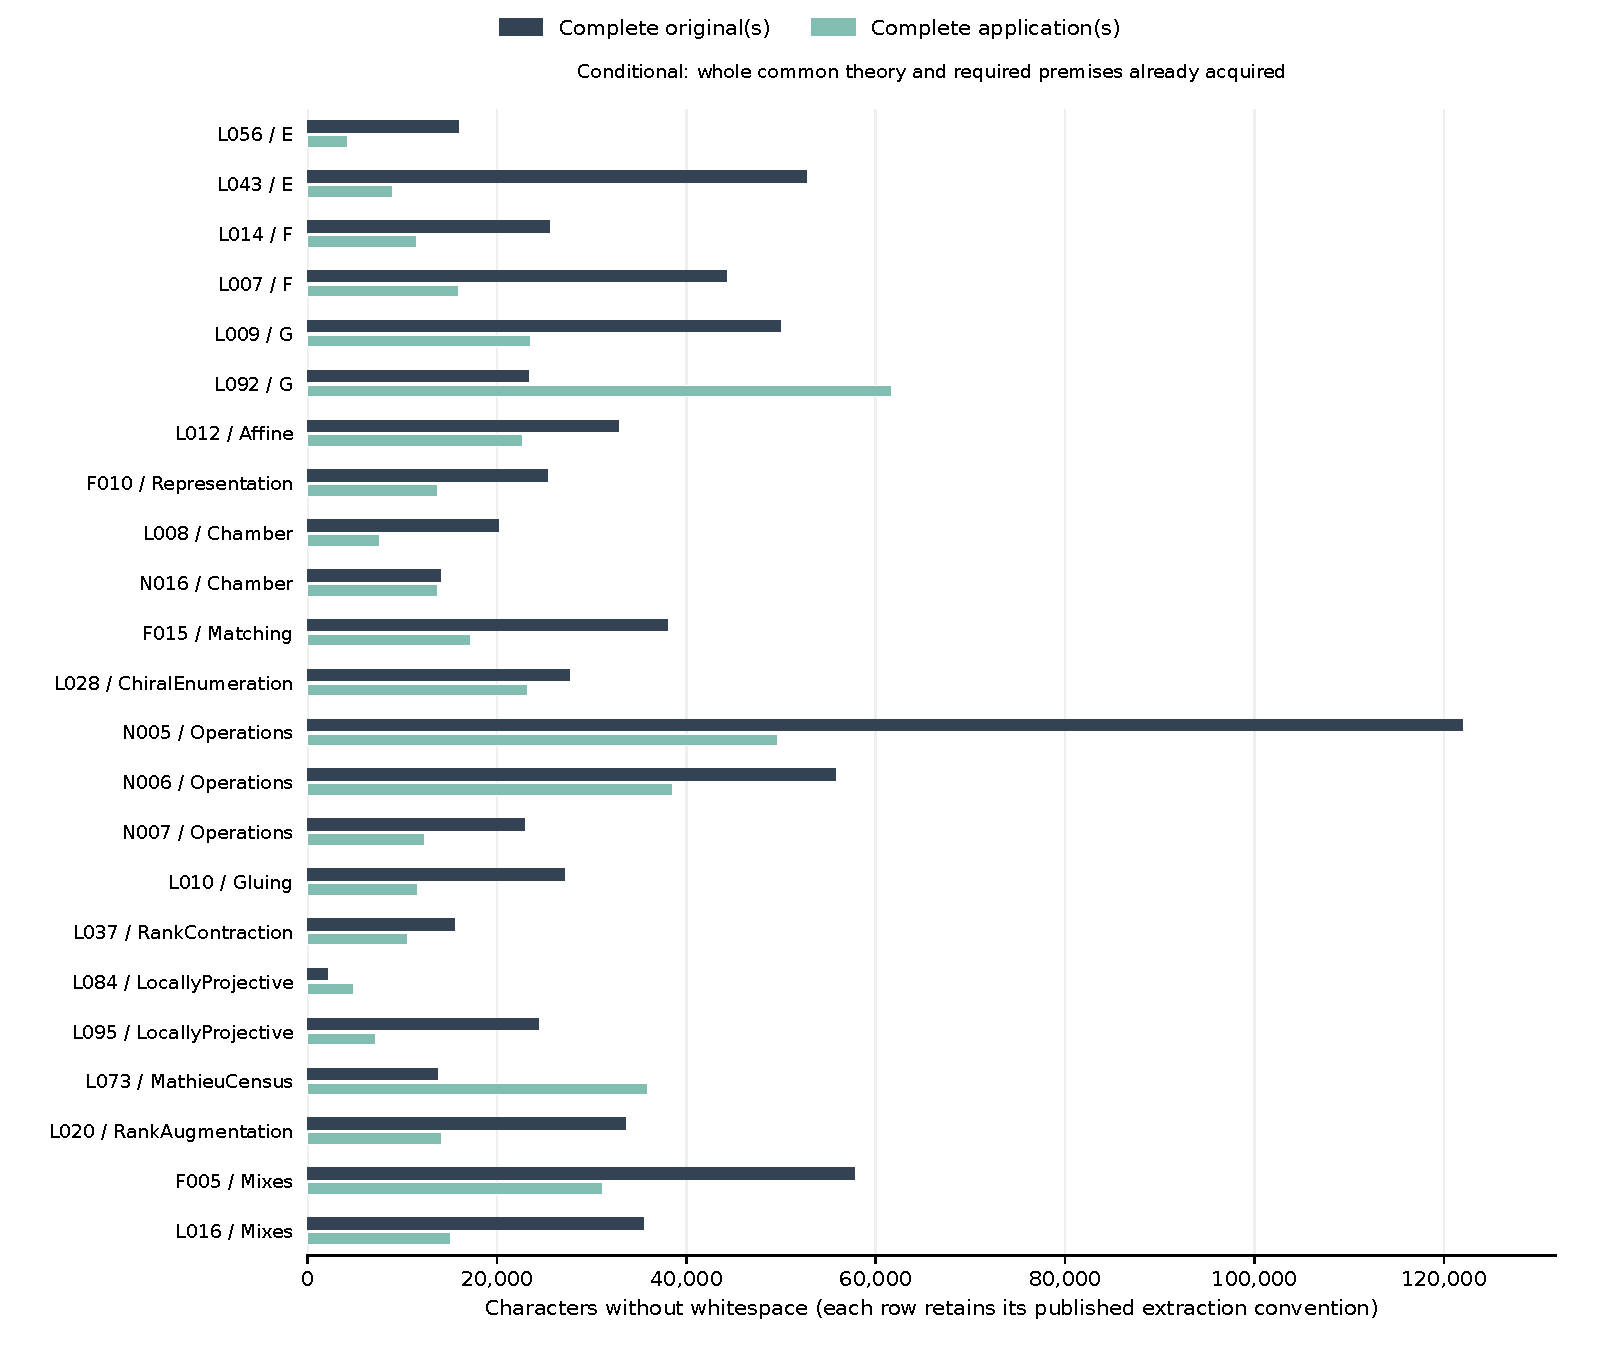
\includegraphics[width=\linewidth]{conditional_2.pdf}\end{center}
\end{document}
